\subsection{Launcher}\label{sec:launcher}
A launcher in Android terminology is an application that provides easy access to other applications present on the system.
When the system is fully booted, the launcher is automatically started and is thus comparable to booting a desktop computer directly to the desktop.

From this point and onwards, when referring to \textit{\launcher} (with capital 'L'), we are drawing attention to the launcher that is part of the \giraf application suite.

The main purpose of \launcher is to provide a user-friendly means of accessing other applications in the \giraf suite, as well as regulating access to these applications.\thilemann{Does this also include native Android apps?} \vagner{It does, but we didnt know that untill sprint 2. Should we therefore write about it here?}

\subsubsection{Motivation for Working with Launcher}
Launcher was originally developed by \citet{launcher2011}, and further refined by \citet{launcher2012}.
On an opening meeting however, the costumer contact persons made us aware that they rarely used Launcher, as it often would crash. \thilemann{Which opening meeting? Sprint meeting?}
They preferred to access the \giraf applications through the Android interface (native launcher).
As mentioned in \cref{sec:sprint1:objectives}, the focus in this sprint is on creating running applications.
Since \launcher was relatively complete based on the development of \citet{launcher2012}, but reported as being unreliable by the customers, an obvious task for the sprint is to make \launcher run reliably.

\subsubsection{Launcher Functionality}
As the \launcher covers multiple tasks in the \giraf project, this section will give a detailed description of its most important activities (screens in the application).\vagner{Should we assume that the reader knows what an activity is in Android context or should we explain it?}
Screenshots of each activity is found in \cref{fig:launcheractivities}.

\begin{figure}[h] % Billeder af draweren i åben og lukket tilstand
\centering
	\begin{subfigure}[b]{.48\textwidth}
	\centering
	
\includegraphics[width=\textwidth, height=3in, keepaspectratio=true] {screenshots-old-giraf/giraf-logoactivity.png}
	\caption{\textit{Logo} activity.}
	\label{fig:launcheractivity:logo}
	\end{subfigure}
	\hfill
	\begin{subfigure}[b]{.48\textwidth}
	\centering
	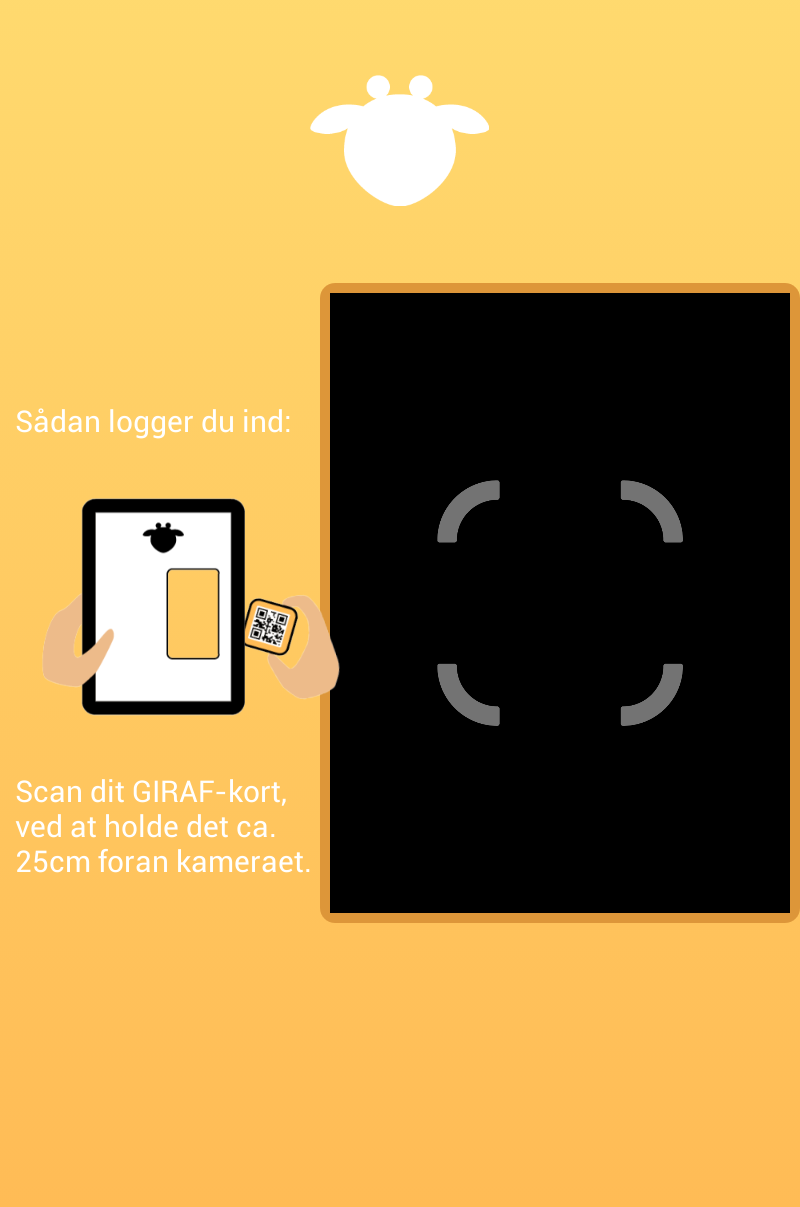
\includegraphics[width=\textwidth, height=3in, keepaspectratio=true] {screenshots-old-giraf/giraf-authenticationactivity.png}
	\caption{\textit{Authentication} activity.}
	\label{fig:launcheractivity:auth}
	\end{subfigure}
	
	\quad % Inserts extra space between rows of subfigures
	
	\begin{subfigure}[b]{.48\textwidth}
	\centering
	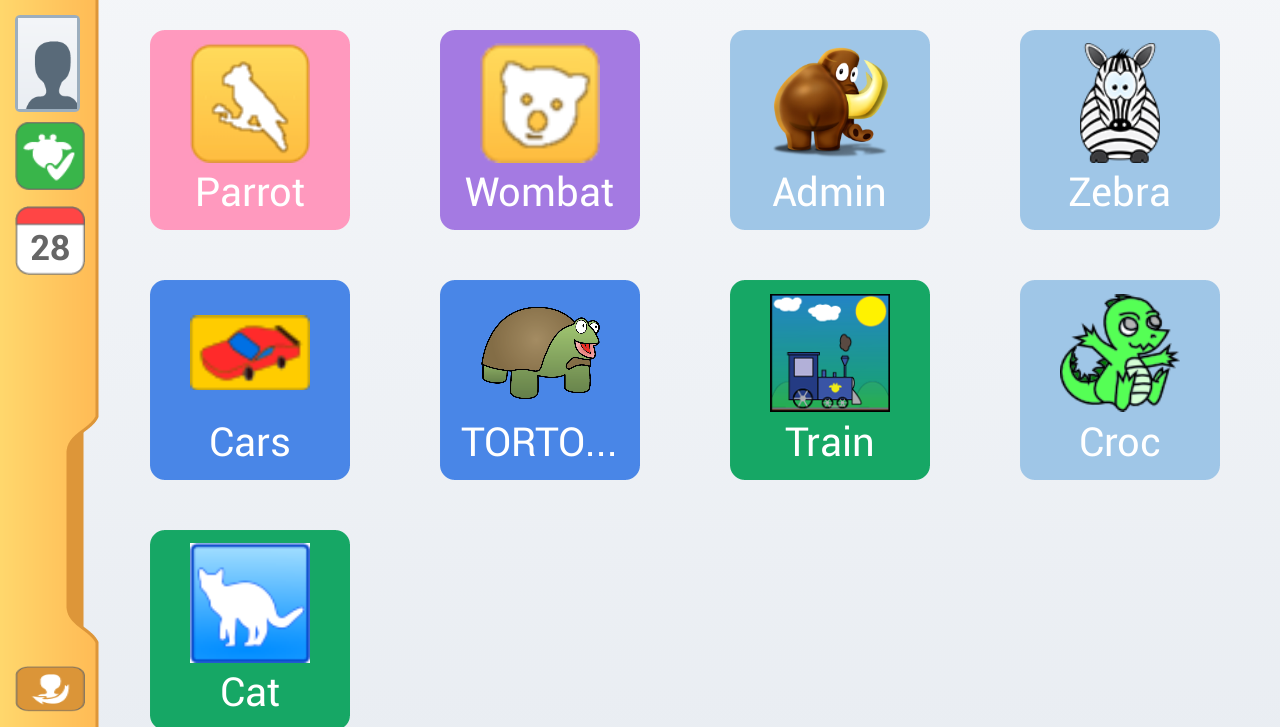
\includegraphics[width=\textwidth]{screenshots-old-giraf/giraf-homeactivity.png}
	\caption{\textit{Home} activity.}
	\label{fig:launcheractivity:home}
	\end{subfigure}
	\begin{subfigure}[b]{.48\textwidth}
	\centering
	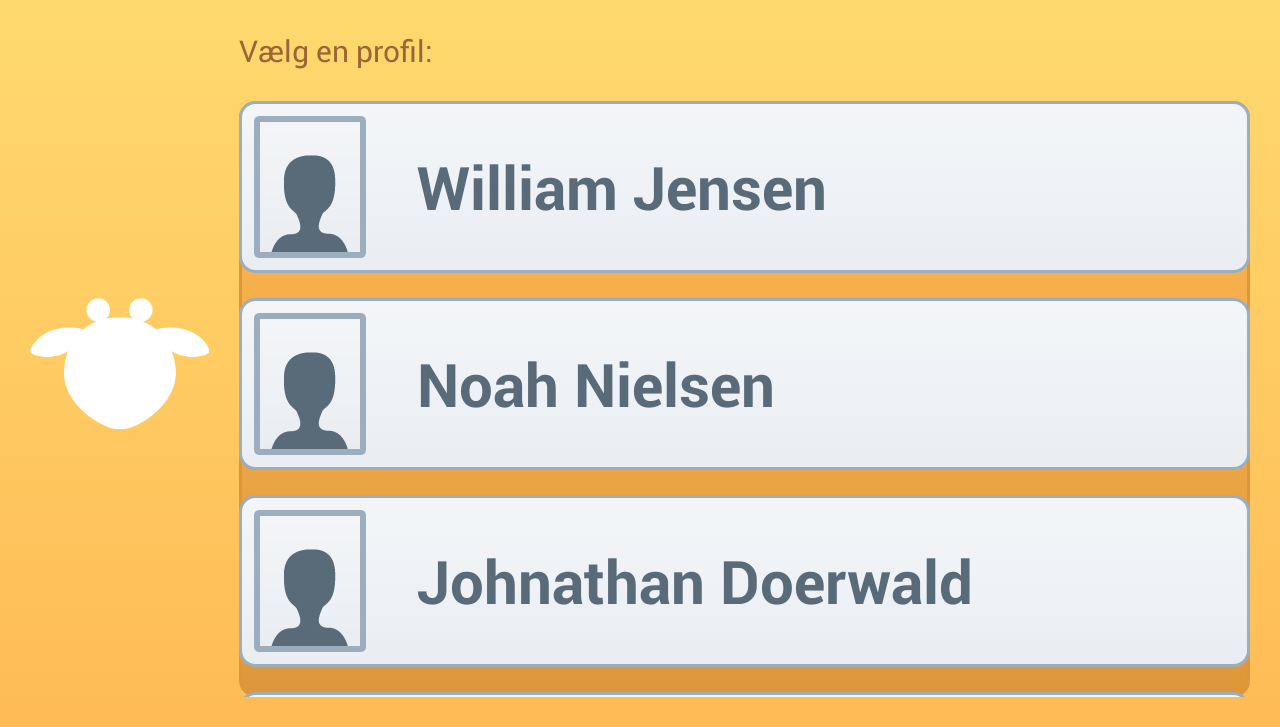
\includegraphics[width=\textwidth]{screenshots-old-giraf/giraf-profileselect.png}
	\caption{\textit{ProfileSelect} activity.}
	\label{fig:launcheractivity:profile}
	\end{subfigure}
\caption{Activities of the \giraf application.}
\label{fig:launcheractivities}
\end{figure}

\paragraph{Logo activity} is only responsible for showing the \giraf logo for a specified amount of time (as seen in \cref{fig:launcheractivity:logo}), and then redirecting the users to the proper activity.
It redirects to Authentication activity if the user is not logged in, or to the Home activity if the user is already logged in.\thilemann{Discuss if fx activities should be written as inline listings.}

\paragraph{Authentication activity} requires the user to authenticate him- or herself before proceeding. 
\citet{launcher2012} describes how user identification is necessary, as the \giraf settings must be able to vary from user to user. 
The report furthermore describes how autistic children might have problems using a traditional user-name and password system. 
Therefore, the authentication activity is based on a QR-scanner, as seen in \cref{fig:launcheractivity:auth}.
Each child and guardian then uses a small brick with their personal QR-code they scan to identify themselves. 
The activity loads the user information from the database, and proceeds to the Home activity.

\paragraph{Home activity} allows the user to launch \giraf applications available to his or her user account. 
The availability of an applications depends on whether the application exists locally on that device, and on whether the user is marked in the database as having proper access rights to that application.
The \textit{Home} activity for a test guardian user is seen in \cref{fig:launcheractivity:home} with the user's installed \giraf applicatons.
Furthermore, a number of widgets allows the user to see the synchronization status of the local database in relation to the remote database, and a widget showing current date. 
There is also a button that allows the user to log out, and return to the Authentication activity.
Finally, there is a colour palette hidden in a drawer component, where the user can change the base colour of each installed application. 
The idea is to make it easier for the children to differentiate between the various applications by being choosing their own colourscheme. 
Ideally the choice of colour should also reflect in the application started from the \launcher, giving the child consistent visual associations throughout \giraf.
The latter is for example implemented in the \textit{Timer} application.\vagner{Add a source to this}\thilemann{Is that necessary?}

\paragraph{Profile Select activity} is started when a guardian launches an application from \launcher. 
It displays a list of all children associated with this guardian (as seen in \cref{fig:launcheractivity:profile}), allowing him or her to choose which child's profile to use when launching the selected application. 
When a child is selected, the application launches, omitting the \textit{Profile Select activity}.